\lstdefinestyle{mystyle}{
    basicstyle=\footnotesize,                
   	captionpos=b,                     
   	numbers=left,                    
   	numbersep=5pt,             
   	tabsize=2
}
\lstset{style=mystyle}
%versi 2 (8-10-2016)
\chapter{Landasan Teori}
\label{chap:teori}
Bab ini akan membahas teori-teori yang akan menjadi dasar dari penelitian ini. Teori yang dibahas yaitu mengenai {\it Javadoc}, {\it Doclet} dan \LaTeX .

\section{Javadoc}
\label{sec:javadoc} 
{\it Javadoc} adalah sebuah {\it tools} yang dimiliki oleh {\it Java} yang berguna untuk mengekstrak informasi dari sekumpulan {\it source file java} menjadi sebuah dokumentasi. Umumnya {\it Javadoc} menghasilkan sekumpulan {\it file} HTML yang mendeskripsikan sebuah {\it class}, {\it interface}, {\it method} dan {\it custom tag}. {\it Javadoc} dapat mengekstraksi informasi tersebut dari sebuah {\it package java}, sebuah {\it file java} atau keduanya. ~\cite{javadoc:01:javadoc}

\subsection{\textit{Processing of source files}}
\label{sec:javadoc}
{\it Javadoc} akan memproses {\it file} yang memiliki akhiran {\it ".java"} dan keseluruhan {\it file} yang terdapat di dalam folder yang sama. {\it Javadoc} dapat mengambil informasi dari 1 atau lebih {\it file java} dan sebuah {\it package}.

{\it Javadoc} dapat memproses sebuah {\it link} secara otomatis yang mengarah kepada sebuah {\it package}, {\it class} dan sebuah nama yang akan didokumentasikan pada saat {\it Javadoc} memprosesnya. {\it Link-link} tersebut berada pada beberapa posisi seperti:
\begin{enumerate}
	\item {\it Declaration} ({\it return types}, {\it argument types}, {\it field types})
	\item Bagian {\it "See Also"} yang dihasilkan oleh {\it tag @see}
	\item {\it In-line text} yang dihasilkan oleh {\it tag {@link}}
	\item {\it Exeption} yang dihasilkan oleh {\it tag @throws}
	\item {\it Link "Specified by"} untuk {\it member} dari sebuah {\it interface}
	\item {\it Link "Override"} untuk {\it member} dari sebuah {\it class}
\end{enumerate}

Dalam mengekstrak informasi yang terdapat dalam sebuah {\it package java} atau beberapa {\it file java} umumnya menghasilkan sebuah dokumentasi standar yang berbentuk {\it file} HTML dan format penulisan yang mengikuti standar {\it Javadoc}, akan tetapi untuk menghasilkan sebuah format dokumentasi yang diingin, dapat menggunakan sebuah {\it doclet} yang disediakan oleh {\it Javadoc}.

\subsection{Terminologi}
\label{sec:terminologi}
Terdapat beberapa istilah yang memiliki arti spesifik dalam konteks {\it Javadoc} sebagai berikut:
\begin{itemize}
	\item {\it Generated Document}\\
	Dokumen yang dihasilkan oleh {\it Javadoc tools} adalah sebuah {\it file} HTML dan dibuat oleh {\it standard doclet}
	\item {\it Name}\\
	Nama dari sebuah perangkat lunak dituliskan dalam bahasa {\it Java} yaitu nama {\it package}, {\it class}, {\it interface}, {\it field}, {\it constructor} atau {\it method}. Nama tersebut dapat berupa informasi lengkapnya seperti {\it java.lang.String.equals(java.lang.Object)} atau informasi pendeknya seperti {\it equals(Object)}
	\item {\it Documented Classes}\\
	Detail dari sebuah {\it class} dan {\it interface} akan didokumentasikan pada saat {\it Javadoc} berjalan. Untuk dapat didokumentasikan, {\it source file} harus tersedia, kemudian nama dari {\it source file} atau nama dari {\it package} tersebut harus diletakkan pada {\it Javadoc command-line}
	\item {\it Included Classes}\\
	{\it Class} dan {\it Interface} akan didokumentasikan pada saat {\it Javadoc} berjalan, hal ini sama seperti {\it Documented Classes}
	\item {\it Excluded Classes}\\
	{\it Class} dan {\it Interface} tidak akan didokumenasikan pada saat {\it Javadoc} berjalan.
	\item {\it Referenced Classes}\\
	{\it Class} dan {\it Interface} yang secara eksplisit disebut oleh {\it class} dan {\it interface} lainnya, seperti {\it return type}, {\it parameter type}, {\it cast type}, {\it extended class}, {\it implemented interface}, {\it imported class}, {\it class} yang digunakan pada {\it method body}, {\it @see}, {\it {@link}}, {\it {@linkplain}} dan {\it {@inheritDoc} tag} 
	\item {\it External Referenced Classes}\\
	{\it Class} yang tidak dihasilkan saat {\it Javadoc} berjalan. Dengan kata lain, {\it class} tersebut tidak diletakkan pada {\it Javadoc command-line}. {\it Links} akan dihasilkan jika sebuah {\it class} mengatakan memiliki {\it external references} atau {\it external link}.
\end{itemize}

\subsection{\textit{Source Files}}
\label{sec:source-files}
{\it Javadoc} akan menghasilkan {\it output} yang berasal dari beberapa tipe {\it file}, yaitu sebagai berikut:
\begin{itemize}
	\item {\it Class Source Code Files}\\
	Setiap {\it class} atau {\it interface} dapat memiliki dokumentasinya masing-masing yang terdapat pada {\it file java}
	\item {\it Package Comment Files}\\
	Setiap {\it package} dapat memiliki dokumentasinya masing-masing yang terdapat pada {\it root} folder kemudian {\it Javadoc} akan menggabungkan {\it file-file} yang terdapat pada {\it root} menjadi sebuah ringkasan. Untuk membuat dokumentasi tersebut, terdapat 2 pilihan yaitu sebuah {\it file} package.html \ref{package} atau sebuah {\it file} package-info.java \ref{package-info}.
	\begin{lstlisting}[language=Html, caption={\it File} package.html, label={package}]
	<html>
	<body>
	Provides the classes necessary to create an applet and the classes
	an applet uses to communicate with its applet context.
	
	@since 1.0
	@see java.awt
	</body>
	</html>
	\end{lstlisting}
	
	\begin{lstlisting}[language=Java, caption={\it File} package-info.java, label={package-info}]
	/**
	 * Provides the classes necessary to create an applet
	 * and the classes an applet uses to communicate
	 * with its applet context.
	 *
	 * @since 1.0
	 * @see java.awt
	 */
	 package java.lang.applet;
	\end{lstlisting}
	Ketika {\it Javadoc} memproses {\it package} tersebut, {\it Javadoc} akan melakukan beberapa langkah yaitu sebagai berikut:
	\begin{enumerate}
		\item Menyalin informasi untuk diproses. Jika {\it file} berupa HTML maka pada bagian {\it <body>} hingga {\it </body>} akan disalin.
		\item Memproses semua {\it tag} pada {\it package} yang ada.
		\item Memasukan teks yang sudah diproses tersebut pada bagian bawah halaman dokumentasi yang dihasilkan.
		\item Salin kalimat pertama pada {\it package} tersebut pada bagian atas halaman dokumentasi
	\end{enumerate}
	\item {\it Overview Comment Files}\\
	Setiap aplikasi atau sekumpulan {\it package} yang akan didokumentasikan akan memiliki dokumentasi {\it overview}. Dokumentasi tersebut dapat dibuat lebih dari 1, jika pada saat pembuatan perangkat lunak menggunakan sekumpulan {\it package} yang berbeda. Untuk membuat sebuah dokumentasi ini, perlu membuat sebuah {\it file} HTML yang umumnya bernama {\it overview.html}. Kemudian {\it Javadoc} akan memproses seperti pada {\it Package Comment Files}
	\item {\it Miscellaneous Unprocessed Files}\\
	{\it File} tersebut dapat berubah sebuah {\it graphic files}, {\it file java} dan sebuah {\it file} HTML.
\end{itemize}

\subsection{\textit{Generated Files}}
\label{sec:generated-files}
Secara {\it default}, {\it Javadoc} akan menggunakan {\it standard doclet} yang akan menghasilkan sebuah dokumentasi berformat HTML. Doclet tersebu akan menghasilkan {\it file} HTML secara terpisah. Terdapat 3 grup yang masing-masing grup memiliki kriterianya sendiri, 3 grup tersebut adalah sebagai berikut:
\begin{itemize}
	\item {\it Basic Content Pages}
	\begin{itemize}
		\item sebuah halaman {\it class} atau {\it interface} ({\it classname}.html) untuk masing-masing {\it class} atau {\it interface} yang akan didokumentasikan
		\item sebuah halaman {\it package} ({\it package-summary.html}) untuk masing-masing {\it package} yang akan didokumentasikan
		\item sebuah halaman {\it overview} ({\it overview-summary.html}) untuk keseluruhan sekumpulan {\it package}. Halaman ini adalah halaman utama yang dihasilkan.
	\end{itemize}
	\item {\it Cross-Reference Pages}
	\begin{itemize}
		\item sebuah halaman hirarki dari {\it class} untuk sekumpulan dari semua {\it package} ({\it overview-tree.html})
		\item sehalaman hirarki dari {\it class} untuk setiap {\it package} ({\it package-tree.html})
		\item sehalaman {\it "use"} ({\it package-use.html}) yang berisikan {\it package}, {\it classes}, {\it methods}, {\it constructors} atau {\it interface}. Jika diberikan sebuah {\it class} bernama A, makan halaman tersebut akan berisikan {\it subclasses} dari A, {\it methods} yang memiliki {\it return} A dan {\it methods} atau {\it constructors} dengan parameter bertipe A.
		\item sebuah halaman {\it deprecated API} ({\it deprecated-list.html}). Halaman ini adalah halaman dari sekumpulan nama yang tidak direkomendasikan untuk digunakan.
		\item sebuah halaman sekumpulan nilai {\it constant} ({\it constant-values.html}) untuk sekumpulan nilai {\it static}.
		\item sebuah halaman {\it serialized form} ({\it serialized-form.html})
		\item sebuah halaman {\it index} ({\it index-*.html}).
	\end{itemize}
	\item {\it Support Files}
	\begin{itemize}
		\item sebuah halaman bantuan ({\it help-doc.html}).
		\item sebuah halaman {\it index} ({\it index.html}) yang membuat sebuah HTML {\it frames}.
		\item beberapa {\it frame file} ({\it *-frame.html}) yang berisi sekumpulan {\it packages}, {\it class} dan {\it interface} dan digunakan pada saat HTML {\it frames} ditampilkan
		\item sebuah {\it file} teks {\it package list} ({\it package-list}).
		\item sebuah {\it style sheet file} ({\it stylesheet.css}) untuk mengontrol warna, jenis {\it font}, ukuran {\it font} dan posisi dari halamanan yang dihasilkan
		\item sebuah {\it doc-files} yang berisikan gambar dan beberapa contoh {\it file java}
	\end{itemize}
\end{itemize}
{\it Javadoc} akan menghasilkan 2 atau 3 HTML {\it frame}. {\it Javadoc} akan membuat minimum {\it frame} yang dibutuhkan. Jika hanya terdapat 1 {\it package}, maka {\it Javadoc} akan membuat 1 {\it frame} yang berisi dari sekumpulan {\it class} pada {\it package} tersebut. Jika terdapat lebih dari 2 {\it package}, maka {\it Javadoc} akan membuat 3 {\it frame} dari sekumpulan {\it package}. Jika {\it class} yang digunakan adalah {\it java.applet.Applet} dan semua dokumentasi yang dihasilkan akan berada pada folder yang bernama {\it apidocs}, struktur {\it file} yang dihasilkan adalah sebagai berikut:
\begin{lstlisting}[caption=Struktur {\it file} yang dihasilkan]
	apidocs						  			  		    Top directory
		index.html											  Initial page that sets up HTML frames
	* overview-summary.html 					  Lists all packages with first sentences summaries
		overview-tree.html							  Lists class hierarchy for all packages
		deprecated-list.html              Lists deprecated API for all packages
   		constant-values.html            Lists values of static fields for all packages
   		serialized-form.html            Lists serialized form for all packages
   * overview-frame.html              Lists all packages, used in upper-left frame
   		allclasses-frame.html           Lists all classes for all packages, used in
   																		lower-left frame
   		help-doc.html                   Lists user help for how these pages are organized
   		index-all.html                  Default index created without -splitindex option
   		index-files                     Directory created with -splitindex option
       		index-<number>.html         Index files created with -splitindex option
   		package-list                    Lists package names, used only for 
   																		resolving external refs
   		stylesheet.css                  HTML style sheet for defining fonts, colors and
   																		positions
   		java                            Package directory
       		applet                      Subpackage directory
            	Applet.html             Page for Applet class
            	AppletContext.html      Page for AppletContext interface
            	AppletStub.html         Page for AppletStub interface
            	AudioClip.html          Page for AudioClip interface
          * package-summary.html    	Lists classes with first sentence summaries
          														for this package
          * package-frame.html      	Lists classes in this package, used in
          														lower left-hand frame
          * package-tree.html       	Lists class hierarchy for this package
            package-use             	Lists where this package is used
            	doc-files               Directory holding image and example files
            	class-use               Directory holding pages API is used
                	Applet.html         Page for uses of Applet class
                	AppletContext.html  Page for uses of AppletContext interface
                	AppletStub.html     Page for uses of AppletStub interface
                	AudioClip.html      Page for uses of AudioClip interface
   		src-html                        Source code directory
       		java                        Package directory
           		applet                  Subpackage directory
                	Applet.html         Page for Applet source code
                	AppletContext.html  Page for AppletContext source code
                	AppletStub.html     Page for AppletStub source code
                	AudioClip.html      Page for AudioClip source code
\end{lstlisting}
\section{Doclet}
\label{sec:doclet}
{\it Doclet} yang terdapat pada {\it Javadoc} dapat digunakan untuk menghasilkan sebuah {\it output Javadoc} yang dapat disesuaikan. Standar {\it doclet} yang dihasilkan oleh {\it Javadoc} adalah dokumentasi dengan format HTML. Selain menghasilkan {\it output} yang dapat disesuaikan, Doclet juga dapat mengekstrak informasi secara spesifik.~\cite{doclet:02:doclet}

\subsection{\textit{Interface-interface} pada Doclet}
\label{sec:interface-doclet}
Berikut adalah beberapa {\it interface} yang terdapat pada {\it Doclet}:
\begin{itemize}
	\item {\verb RootDoc }
	sebuah {\it interface} yang menyatakan sebuah {\it root} dari perangkat lunak yang dibuat. Dari {\it root} tersebut semua informasi dapat diekstrak. {\it Method-method} yang digunakan adalah sebagai berikut
	\begin{itemize}
		\item {\verb classes() }\\
		{\it Method} ini akan mengembalikan sejumlah {\it class} dan {\it interface} pada {\it package}
	\end{itemize}
	\item {\verb ClassDoc }
	sebuah {\it interface} yang menyatakan informasi dari sebuah {\it class}. Informasi tersebut dapat berupa nama {\it class}, nama {\it method} dan {\it tag}. {\it Method-method} yang digunakan adalah sebagai berikut
	\begin{itemize}
		\item {\verb name() }\\
		{\it Method} ini akan mengembalikan sebuah nama {\it class} atau {\it interface} pada {\it package}
		\item {\verb commentText() }\\
		{\it Method} ini akan mengembalikan sebuah informasi dari deskripsi {\it class}
		\item {\verb methods() }\\
		{\it Method} ini akan mengembalikan sebuah {\it array of methods} 
	\end{itemize}
	\item {\verb MethodDoc }
	sebuah {\it interface} yang menyatakan informasi dari sebuah {\it method}. {\it Method-method} yang digunakan adalah sebagai berikut
	\begin{itemize}
		\item {\verb name() }\\
		{\it Method} ini akan mengembalikan sebuah nama {\it method}
		\item {\verb modifiers() }\\
		{\it Method} ini akan mengembalikan sebuah {\it access modifier} dari sebuah {\it method}
		\item {\verb returnType() }\\
		{\it Method} ini akan mengembalikan sebuah {\it return type} dari sebuah {\it method}
		\item {\verb flatSignature() }\\
		{\it Method} ini akan mengembalikan {\it signature} dari sebuah {\it method}. Jika terdapat {\it Method} dengan parameter (String x, int y), maka akan mengembalikan (String, int)
	\end{itemize}
	\item {\verb ParamTag }
	sebuah {\it interface} yang menyatakan informasi dari sebuah {\it Tag} parameter. {\it Method-method} yang digunakan adalah sebagai berikut
	\begin{itemize}
		\item {\verb name() }\\
		{\it Method} ini akan mengembalikan sebuah {\it tag @param} 
		\item {\verb parameterName() }\\
		{\it Method} ini akan mengembalikan sebuah nama parameter dari sebuah {\it method}
		\item {\verb parameterComment() }\\
		{\it Method} ini akan mengembalikan sebuah deskripsi dari parameter yang terdapat pada {\it method}
	\end{itemize}
\end{itemize}

\subsection{Penggunaan Doclet}
\label{sec:penggunaan-doclet}
Doclet dapat menghasilkan sebuah {\it output Javadoc} yang dapat disesuaikan. Penggunaan {\it Doclet} API dapat mengekstrak bermacam-macam informasi seperti nama {\it class}, nama {\it method}, deskripsi singkat untuk sebuah parameter dari sebuah {\it method} hingga {\it return type} dari {\it method}.

Berikut adalah langkah-langkah untuk menggunakan {\it doclet}:
\begin{enumerate}
	\item Membuat sebuah {\it class} pada {\it java} sebagai {\it doclet}. {\it class java} tersebut harus meng-{\it import}  \verb com.sun.javadoc.*  untuk menggunakan {\it doclet} API.
	\item {\it Doclet} tersebut diawali dengan sebuah {\it method} \verb public  \verb static  \verb boolean  \verb start  yang memiliki parameter \verb RootDoc .
	\item {\it Compile doclet} tersebut dengan menggunakan {\it compiler} Java 2 SDK yaitu {\it javac} pada {\it command prompt(Windows)}/{\it terminal(Linux)}.
	\item Jalankan {\it Javadoc} menggunakan \verb -doclet  {\it \textbf{startingclass}} {\it option} untuk menghasilkan {\it output} yang telah disesuaikan, dimana {\it \textbf{startingclass}} adalah sebuah {\it class} yang sudah dibuat pada langkah 1.
\end{enumerate}

{\it File doclet} API terdapat pada direktori {\it folder jdk} yang ter-{\it install} pada komputer pada {\it subfolder}  \verb lib\tools.jar .{\it doclet} yang sudah dibuat harus di-{\it compile} menggunakan {\it file}  \verb tools.jar  dan menambahkan {\it option}  \verb -classpath  setelah {\it command}  \verb javac . Jika tidak menggunakan {\it option}  \verb -doclet  , {\it Javadoc} akan menghasilkan {\it output} standar yaitu berupa {\it file} HTML.

{\it Package}  \verb com.sun.javadoc  terdiri {\it interface} yang mendefinisikan {\it doclet} API dan sedangkan {\it file}  \verb tools.jar  berisikan {\it interface-interface} tersebut dan juga berisikan {\it private package} dengan {\it class-class} yang mengimplementasi {\it interface} tersebut serta {\it file} tools.jar berisikan pula {\it class-class} yang mengimplementasi sebuah standar {\it doclet}.

\begin{lstlisting}[language=Java, caption={\it class} ListClass.java]
	import com.sun.javadoc.*;

	public class ListClass {
		public static boolean start(RootDoc doc) {
			ClassDoc[] classes = doc.classes();
			for(int i=0, i < classes.length; i++) {
				System.out.println(classes[i]);
			}
			return true;
		}
	}
\end{lstlisting}
Potongan {\it program} diatas adalah sebuah {\it doclet} sederhana untuk menampilkan nama-nama {\it class} pada {\it file java}. Hal pertama yang harus dilakukan adalah meng-{\it import package}  \verb com.sun.javadoc.* , kemudian membuat sebuah {\it method} \verb public  \verb static  \verb boolean  \verb start  dengan parameter sebuah  \verb RootDoc  doc  yang akan menampung sekumpulan {\it file java} yang akan diproses.  \verb ClassDoc  pada {\it method} tersebut akan menampung nama-nama {\it class} yang terdapat pada variabel  \verb doc  dengan menggunakan {\it method}  \verb classes() .

\section{\LaTeX}
\label{sec:latex}
\LaTeX\ adalah sebuah bahasa {\it markup} untuk sistem penulisan dokumen yang dikembangkan oleh Leslie B. Lamport dan dirilis pada tahun 1985~\cite{latex:03:latex}.  \LaTeX\ Memiliki filosofi WYMIWYG ({\it What you Mean Is What You Get}) yang berarti sesuatu yang ditulis akan berdasarkan arti dari hal tersebut. Oleh karena itu, untuk menambahkan suatu perintah pada dokumen yang sedang ditulis perlu menambahkan suatu {\it command}. {\it Command} adalah kata spesial yang menentukan suatu sifat pada \LaTeX . Hampir semua {\it command} pada \LaTeX\ selalu diawali dengan tanda '$\backslash$' dan beberapa {\it command} memiliki {\it parameter}. {\it Parameter} diawali dengan tanda kurung kurawal buka dan diakhiri dengan kurung kurawal tutup (\{...\}). File \LaTeX\ memiliki ekstensi .tex.

Untuk menulis dokumen pada \LaTeX\ dibutuhkan beberapa {\it command} yang wajib ada dalam sebuah dokumen, yaitu:
\begin{enumerate}
	\item \texttt{\string\documentclass[option]\{class\}}\\
	Digunakan untuk menentukan jenis dokumen yang {\it layout} dokumen. Bagian {\it option} dapat dikosongkan atau dapat digunakan untuk menyimpan pilihan pengaturan {\it layouting}. Pada Bagian {\it class} digunakan untuk menentukan tipe dokumen yang akan dibuat.
	\item \texttt{\string\maketitle}\\
	Digunakan untuk menampilkan halaman judul. Biasanya halaman judul akan memuat judul dokumen, nama pengarang dan tanggal pembuatan dokumen. Judul dokumen, nama pengarang dan tanggal pembuatan dapat ditampilkan dengan menambahkan perintah \texttt{\string\title\{judul\}}, \texttt{\string\author\{nama\}} dan \texttt{\string\date\{tanggal\}}.
	\item \texttt{\string\begin\{document\}}\dots\texttt{\string\end\{document\}}\\
	Digunakan untuk mengawali dan mengakhiri sebuah dokumen.
	\item \texttt{\string\section\{section\}}\\
	Digunakan untuk menampilkan subbab sebuah dokumen.
	\item \texttt{\string\begin\{enumerate\}}\dots\texttt{\string\end\{enumerate\}}\\
	Digunakan untuk menampilkan {\it ordered list}. {\it List} ini akan menampilkan angka yang terurut. Di dalam {\it list} ini terdapat {\it command} \texttt{\string\item} untuk menambahkan isi dari {\it list} tersebut.
\end{enumerate}

%\section{Template Skripsi FTIS UNPAR}
%\label{sec:template}
 
%Akan dipaparkan bagaimana menggunakan template ini, termasuk petunjuk singkat membuat referensi, gambar dan tabel.
%Juga hal-hal lain yang belum terpikir sampai saat ini. 
 
%\dtext{15-16}

%\subsection{Tabel}  
%Berikut adalah contoh pembuatan tabel. 
%Penempatan tabel dan gambar secara umum diatur secara otomatis oleh \LaTeX{}, perhatikan contoh di file bab2.tex untuk melihat bagaimana cara memaksa tabel ditempatkan sesuai keinginan kita.

%Perhatikan bawa berbeda dengan penempatan judul gambar gambar, keterangan tabel harus diletakkan di atas tabel!!
%Lihat Tabel~\ref{tab:contoh1} berikut ini:

%\begin{table}[H] %atau h saja untuk "kira kira di sini"
%	\centering 
%	\caption{Tabel contoh}
%	\label{tab:contoh1}
%	\begin{tabular}{cccc}
%		\toprule
%		& $v_{start}$ & $\mathcal{S}_{1}$ & $v_{end}$\\
%
%		\midrule
%		$\tau_{1}$ & 1 & 12& 20\\
%		$\tau_{2}$ & 1 &  & 20\\
%		$\tau_{3}$ & 1 & 9 & 20\\
%		$\tau_{4}$ & 1 &  & 20\\
%
%		\bottomrule
%		
%	\end{tabular} 
%\end{table}
%Tabel~\ref{tab:cthwarna1} dan Tabel~\ref{tab:cthwarna2} berikut ini adalah tabel dengan sel yang berwarna dan ada dua tabel yang bersebelahan. 
%\begin{table}[H]
%	\begin{minipage}[c]{0.49\linewidth}
%		\centering
%		\caption{Tabel bewarna(1)}
%		\label{tab:cthwarna1}
%		\begin{tabular}{ccccc}
%			\toprule
%			 & $v_{start}$ & $\mathcal{S}_{2}$ & $\mathcal{S}_{1}$ & $v_{end}$\\
%			
%			\midrule
%			$\tau_{1}$ & 1 & 5 \cellcolor{green}& 12& 20\\
%			$\tau_{2}$ & 1 & 8 \cellcolor{green}& & 20\\
%			$\tau_{3}$ & 1 & 2/8/17 \cellcolor{green}& 9 & 20\\
%			$\tau_{4}$ & 1 & \cellcolor{red}& & 20\\
%			
%			\bottomrule
%
%		\end{tabular}
%	\end{minipage}
%	\begin{minipage}[c]{0.49\linewidth}
%		
%		\centering 
%		\caption{Tabel bewarna(2)}
%		\label{tab:cthwarna2}
%		\begin{tabular}{ccccc}
%			\toprule
%			 & $v_{start}$ & $\mathcal{S}_{1}$ & $\mathcal{S}_{2}$ & $v_{end}$\\
%			
%			\midrule
%			$\tau_{1}$ & 1 & 12& 5 \cellcolor{red} &20\\
%			$\tau_{2}$ & 1 &  &  8 \cellcolor{green} &20\\
%			$\tau_{3}$ & 1 & 9 & 2/8/17 \cellcolor{green} &20\\
%			$\tau_{4}$ & 1 &   & \cellcolor{red} &20\\
%			
%			\bottomrule
%		
%		\end{tabular}
%	\end{minipage}
%\end{table}

 
%\subsection{Kutipan}
%\label{subs:kutipan} 
%Berikut contoh kutipan dari berbagai sumber, untuk keterangan lebih lengkap, silahkan membaca file referensi.bib yang disediakan juga di template ini.
%Contoh kutipan:
%\begin{itemize}
%	\item Buku:~\cite{berg:08:compgeom} 
%	\item Bab dalam buku:~\cite{kreveld:04:GIS}
%	\item Artikel dari Jurnal:~\cite{buchin:13:median}
%	\item Artikel dari prosiding seminar/konferensi:~\cite{kreveld:11:median}
%	\item Skripsi/Thesis/Disertasi:~\cite{lionov:02:animasi}~\cite{wiratma:10:following}~\cite{wiratma:22:later}
%	\item Technical/Scientific Report:~\cite{kreveld:07:watertight}
%	\item RFC (Request For Comments):~\cite{RFC1654}
%	\item Technical Documentation/Technical Manual:~\cite{Z.500}~\cite{unicode:16:stdv9}~\cite{google:16:and7}
%	\item Paten:~\cite{webb:12:comm}
%	\item Tidak dipublikasikan:~\cite{wiratma:09:median}~\cite{lionov:11:cpoly}
%	\item Laman web:~\cite{erickson:03:cgmodel}  
%	\item Lain-lain:~\cite{agung:12:tango}
%\end{itemize}    
  
%\subsection{Gambar}

%Pada hampir semua editor, penempatan gambar di dalam dokumen \LaTeX{} tidak dapat dilakukan melalui proses {\it drag and drop}.
%Perhatikan contoh pada file bab2.tex untuk melihat bagaimana cara menempatkan gambar.
%Beberapa hal yang harus diperhatikan pada saat menempatkan gambar:
%\begin{itemize}
%	\item Setiap gambar {\bf harus} diacu di dalam teks (gunakan {\it field} {\sc label})
%	\item {\it Field} {\sc caption} digunakan untuk teks pengantar pada gambar. Terdapat dua bagian yaitu yang ada di antara tanda $[$ dan $]$ dan yang ada di antara tanda $\{$ dan $\}$. Yang pertama akan muncul di Daftar Gambar, sedangkan yang kedua akan muncul di teks pengantar gambar. Untuk skripsi ini, samakan isi keduanya.
%	\item Jenis file yang dapat digunakan sebagai gambar cukup banyak, tetapi yang paling populer adalah tipe {\sc png} (lihat Gambar~\ref{fig:ularpng}), tipe {\sc jpg} (Gambar~\ref{fig:ularjpg}) dan tipe {\sc pdf} (Gambar~\ref{fig:ularpdf})
%	\item Besarnya gambar dapat diatur dengan {\it field} {\sc scale}.
%	\item Penempatan gambar diatur menggunakan {\it placement specifier} (di antara tanda  $[$ dan $]$ setelah deklarasi gambar.
%	Yang umum digunakan adalah {\bf H} untuk menempatkan gambar {\bf sesuai} penempatannya di file .tex atau  {\bf h} yang berarti "kira-kira" di sini. \\
%	Jika tidak menggunakan {\it placement specifier}, \LaTeX{} akan menempatkan gambar secara otomatis untuk menghindari bagian kosong pada dokumen anda.
%	Walaupun cara ini sangat mudah, hindarkan terjadinya penempatan dua gambar secara berurutan. 	
%	\begin{itemize}
%		\item Gambar~\ref{fig:ularpng} ditempatkan di bagian atas halaman, walaupun penempatannya dilakukan setelah penulisan 3 paragraf setelah penjelasan ini.
%		\item Gambar~\ref{fig:ularjpg} dengan skala 0.5 ditempatkan di antara dua buah paragraf. Perhatikan penulisannya di dalam file bab2.tex!
%		\item Gambar~\ref{fig:ularpdf} ditempatkan menggunakan {\it specifier} {\bf h}.
%	\end{itemize}
%\end{itemize}
 
%\dtext{17-18}
%\begin{figure} 
%	\centering  
%	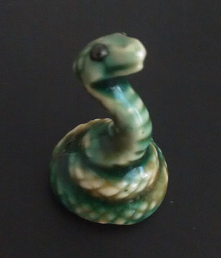
\includegraphics[scale=1]{ular-png}  
%	\caption[Gambar {\it Serpentes} dalam format png]{Gambar {\it Serpentes} dalam format png} 
%	\label{fig:ularpng} 
%\end{figure} 

%\dtext{19-20}
%\begin{figure}[H]
%	\centering  
%	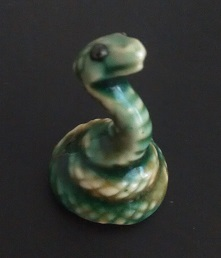
\includegraphics[scale=0.5]{ular-jpg}  
%	\caption[Ular kecil]{Ular kecil} 
%	\label{fig:ularjpg} 
%\end{figure} 
%\dtext{21-22}

%\begin{figure}[ht] 
%	\centering  
%	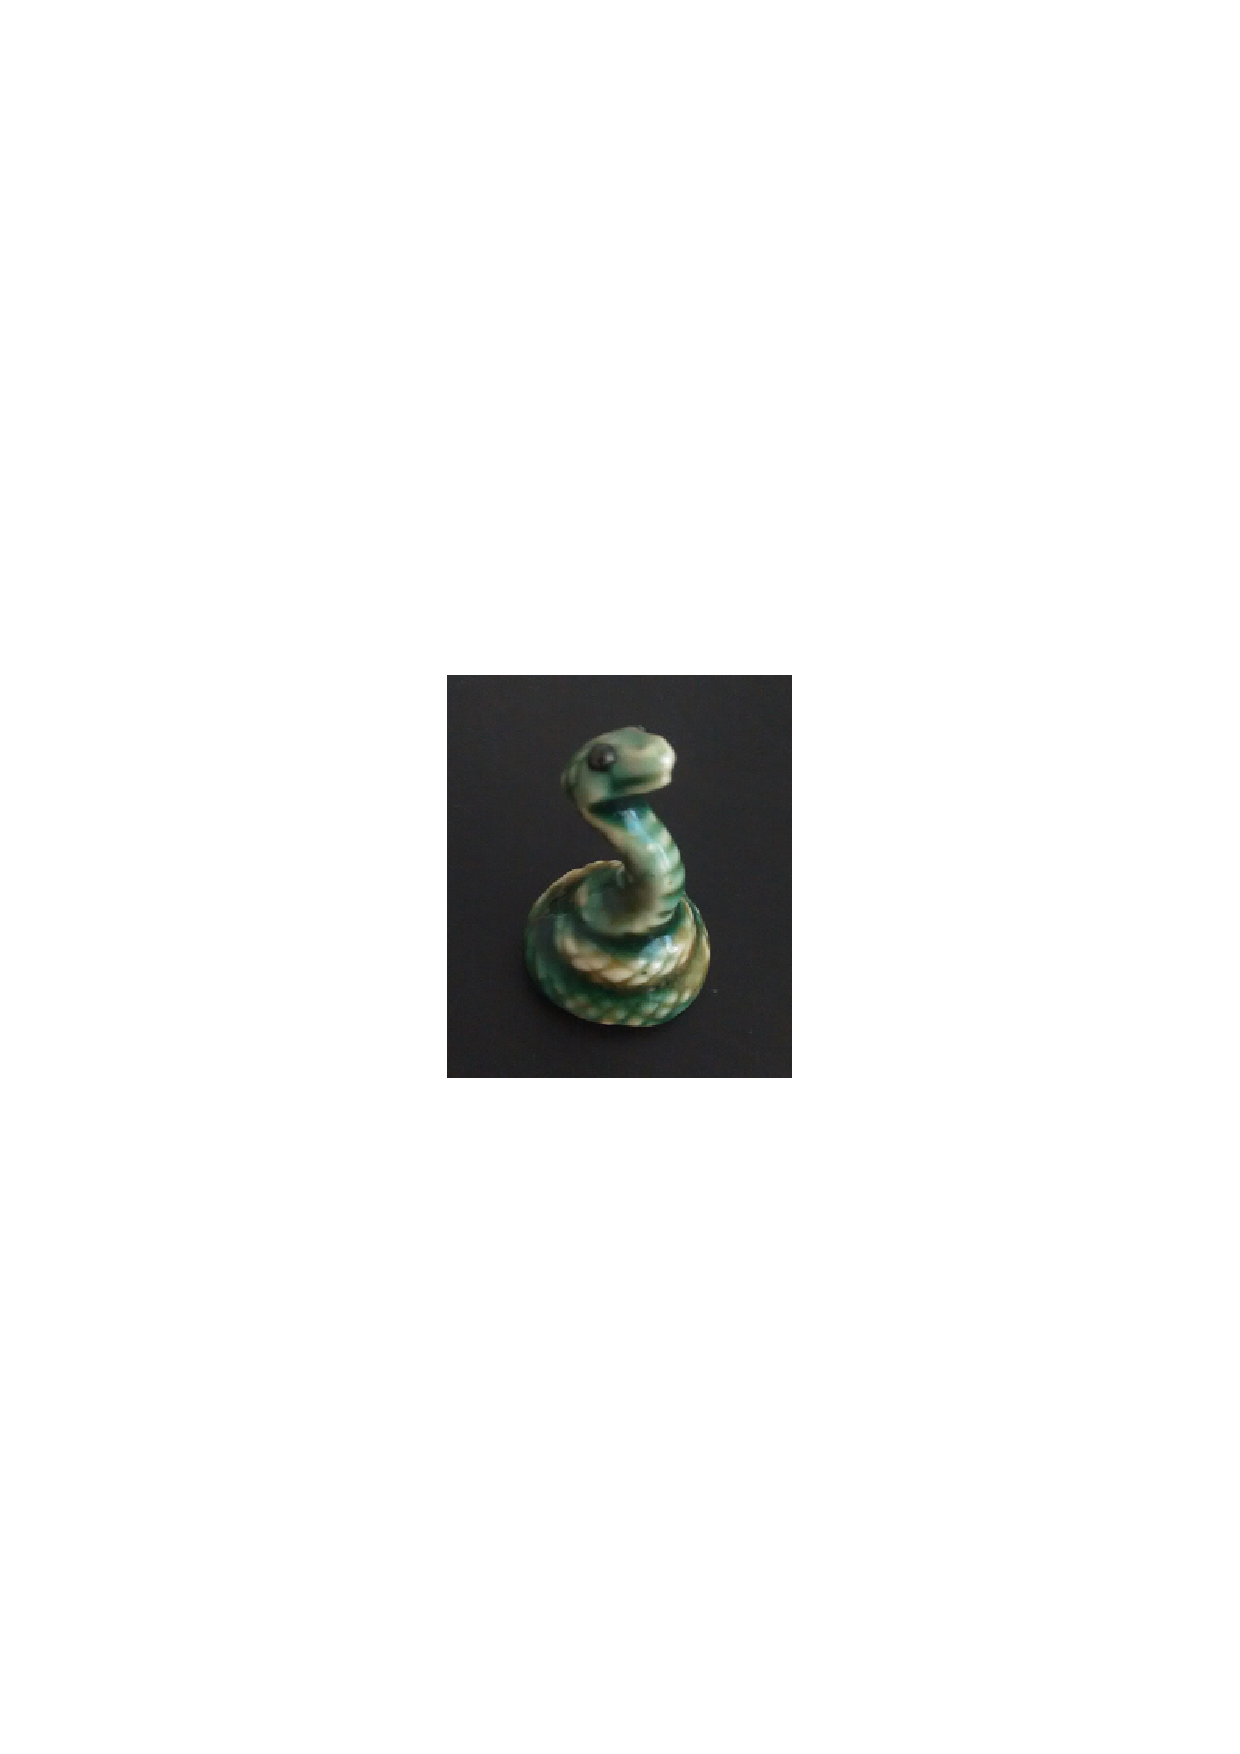
\includegraphics[scale=1]{ular-pdf}  
%	\caption[ {\it Serpentes} betina]{ {\it Serpentes} jantan} 
%	\label{fig:ularpdf} 
%\end{figure}
 
